\chapter{Replication report}
\label{chapter2}

\section{Anomaly Detection Replication}

This section presents a replication and analysis of a lightweight anomaly detection approach proposed for edge-based Kubernetes clusters. The goal is not only to reproduce reported behaviour, but also to evaluate its robustness under realistic edge preprocessing conditions.

\subsection{Introduction}

Edge Kubernetes environments demand monitoring solutions that are both effective and lightweight. Since edge computing exists to achieve low latency and high bandwidth, any added computation for monitoring must be carefully optimised to operate within resource constraints, intermittent connectivity, geographic distribution, and the need for autonomous operation \cite{rasouli2025false}.

Anomaly detection supports lightweight monitoring by enabling real-time decisions about node health. By identifying abnormal behaviour locally, edge nodes can selectively transfer only relevant data, reducing network load and storage cost. Additional benefits include improved security posture, predictive maintenance capabilities, context-aware resource management, and greater system autonomy \cite{fritzsche2024lightweight}.

For anomaly detection in this context, K-means and the Negative Selection Algorithm (NSA) offer complementary strengths. K-means provides computationally simple clustering-based analysis on large unlabelled datasets, while NSA offers lightweight multi-dimensional classification that is well-suited to the diverse operating conditions of edge environments \cite{fritzsche2024lightweight}.

\subsection{Method Overview}

Fritzsche et al.\ demonstrated that a combination of K-means and NSA detection achieves effective anomaly detection in edge Kubernetes clusters \cite{fritzsche2024lightweight}. This section replicates their approach under controlled conditions to evaluate detector behaviour and sensitivity to preprocessing.

The NSA algorithm takes as input three sets: a \textit{self} set representing normal behaviour, a \textit{monitor} set of observations to classify, and a \textit{detector} set generated during training. Given a maximum detector count $n$, detectors are randomly generated in feature space and retained only if they do not match any self-region data point. At runtime, each observation in the monitor set is classified as \textit{self} or \textit{non-self} based on proximity to detectors.

NSA is well-suited to edge environments because it requires only normal-behaviour training data (one-class learning), imposes minimal computational overhead at inference time, and naturally adapts to multi-dimensional feature spaces without requiring labelled anomaly examples.

\subsection{Experimental Setup (offline)}

An offline evaluation was conducted to isolate detector behaviour from runtime cluster effects, enabling controlled algorithm evaluation and sensitivity analysis independent of network variability or collection artefacts.

\subsubsection{Metrics}

Synthetic edge metrics were generated using normal distributions to simulate CPU, memory, and network utilisation under typical operating conditions. Two modes of anomaly injection were used---subtle (transient point anomalies) and sustained (prolonged multi-dimensional deviations)---which present varying sensitivity to preprocessing.

Subtle point anomalies were designed to emulate transient workload disturbances common in edge environments. However, after rolling-window smoothing and feature normalisation, these anomalies became geometrically embedded within the normal data distribution. As a result, no distinct non-self region emerged, rendering NSA incapable of detecting such deviations by design.

In contrast, sustained multi-dimensional anomalies introduce prolonged deviations in system behaviour, forming a distinct abnormal operating regime. When excessive smoothing is avoided, this regime remains geometrically separable from normal workloads, allowing NSA to successfully identify non-self regions.

\subsubsection{Preprocessing}

Preprocessing was completed to achieve edge realism. Edge monitoring systems must trade precision for stability, bandwidth efficiency, and robustness.

Rolling-window smoothing was applied to each resource metric to reflect realistic edge telemetry behaviour, where lightweight monitoring systems aggregate measurements over short intervals to suppress noise and reduce communication overhead. This approach stabilises metric trends while preserving sustained workload changes relevant for scheduling decisions.

Feature normalisation was applied to ensure scale invariance across heterogeneous resource metrics, enabling fair distance-based comparison between CPU, memory, and network utilisation. This reflects standard practice in ML-driven resource management pipelines and prevents dominance by high-magnitude features.

While such preprocessing improves robustness and reflects realistic edge monitoring constraints, it also reduces the geometric separability of subtle anomalies, highlighting a fundamental trade-off between noise suppression and anomaly detectability.

\subsubsection{NSA Configuration}

All NSA parameters were held constant across experiments to ensure fair comparison.

\begin{table}[h]
    \centering
    \begin{tabular}{ll}
        \hline
        \textbf{Parameter} & \textbf{Value} \\
        \hline
        Detector count & 200 \\
        Detector radius & 1.5 \\
        Feature space & 3-dimensional (CPU, memory, network) \\
        Training type & Normal-only (one-class) \\
        \hline
    \end{tabular}
    \caption{NSA configuration parameters for offline evaluation.}
    \label{tab:nsa-params}
\end{table}

\subsection{Evaluation Methodology}

Point-wise detection was used to discover individual spikes, which is suitable for scheduler evaluation since it gives high granularity and precision, resulting in the exact identification of decision successes and failures. Precision and recall metrics provided a balanced evaluation; measuring both the accuracy of the detected nodes and the coverage of total positive nodes found.  

The results were interpreted by calculating the distance from the normal of each node that was detected to decide whether it was located in the self or non-self region. If a large proportion of detected nodes were located in the self region, this signaled over sensitivity to the preprocessing pipeline.

\subsection{Results and Analysis}

\subsubsection{Dataset A: Subtle Anomalies}


\begin{table}[h]
    \centering
    \begin{tabular}{ll}
        \hline
        \textbf{Metric} & \textbf{Value} \\
        \hline
        Distance from normal & 0.25 \\
        Precision & 0.00 \\
        Recall & 1.00 \\
        \hline
    \end{tabular}
    \caption{NSA results on Dataset A: subtle point anomalies.}
    \label{tab:results-subtle}
\end{table}

The subtle anomalies were geometrically embedded within the normal distribution after preprocessing, leaving no distinct non-self region for NSA detectors to cover. While recall reached 1.0 (all points were flagged), precision was 0.0, indicating that the detector could not distinguish anomalous points from normal behaviour.

\subsubsection{Dataset B: Sustained Anomalies (default window size)}

\begin{table}[h]
    \centering
    \begin{tabular}{ll}
        \hline
        \textbf{Metric} & \textbf{Value} \\
        \hline
        Distance from normal & 0.34 \\
        Precision & 0.00 \\
        Recall & 1.00 \\
        \hline
    \end{tabular}
    \caption{NSA results on Dataset B with default window size.}
    \label{tab:results-sustained-default}
\end{table}

Despite the anomalies being stronger and more prolonged than in Dataset A, excessive smoothing from the default rolling window collapsed their separability. The distance from normal (0.34) was marginally higher than Dataset A but still insufficient for NSA to establish a meaningful non-self boundary.

\subsubsection{Dataset B: Sustained Anomalies (window size = 2)}

\begin{table}[h]
    \centering
    \begin{tabular}{ll}
        \hline
        \textbf{Metric} & \textbf{Value} \\
        \hline
        Distance from normal & 1.93 \\
        Precision & 0.48 \\
        Recall & 1.00 \\
        \hline
    \end{tabular}
    \caption{NSA results on Dataset B with reduced window size (w=2).}
    \label{tab:results-sustained-w2}
\end{table}

With the reduced window size, the distance from normal increased substantially to 1.93, confirming that a geometrically distinct non-self region emerged. NSA achieved precision of 0.48 while maintaining perfect recall, indicating that the detector successfully identified all anomalous periods albeit with some false positives during transitional phases. This result validates that NSA performs as expected when its core assumption---geometric separability between normal and anomalous behaviour---is preserved through appropriate preprocessing choices.

\section{Online Telemetry Replication}

\subsection{Environment Setup}

The experimental cluster was provisioned on Google Cloud using three virtual machines in the \texttt{europe-west2-c} zone: one \texttt{e2-medium} instance serving as the control plane and two \texttt{e2-small} instances acting as worker nodes. K3s was used as the Kubernetes distribution in place of the full upstream package. As described in Section~\ref{chapter1}, K3s is designed specifically for resource-constrained and remote environments, reducing the operational footprint through a single-binary deployment, an embedded datastore, automated TLS management, and minimal external dependencies. This makes it a closer approximation of realistic edge cluster hardware than a standard Kubernetes installation on cloud VMs.

Netdata was selected as the telemetry platform because it is built for edge-first deployment: it delivers per-second metric precision, maintains a minimal CPU and memory footprint during collection, and operates autonomously when upstream connectivity is interrupted. Netdata agents run on each node, streaming metrics to a parent instance on the control node for centralised collection. The following metrics are recorded per node at a one-second polling interval: CPU usage decomposed into user-space and kernel-space components, RAM utilisation, and network traffic separated into bytes received and bytes sent.

Figure~\ref{fig:online-system-architecture} presents the deployed online telemetry architecture used for the replication.

\begin{figure}[htbp]
    \centering
    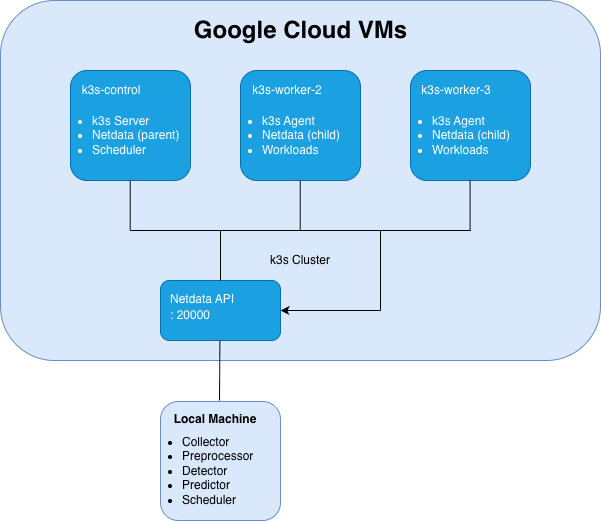
\includegraphics[width=0.95\textwidth]{../docs/system-architecture.png}
    \caption{System architecture of the online telemetry replication testbed (K3s control plane, worker nodes, and Netdata telemetry flow).}
    \label{fig:online-system-architecture}
\end{figure}

\subsection{Experiment Design}

The experiment was structured as six sequential phases, each lasting 120 seconds. The phases progressed from a normal-load baseline, through four distinct stress injection scenarios, to a recovery period. For each stress phase, the \texttt{stress} tool was invoked on the target node via SSH, injecting load into specific resource subsystems. The start and end timestamps of each phase were recorded automatically to enable programmatic labelling of the collected dataset.

Metrics were collected from all three nodes throughout the experiment, including the control node. Although the control node is excluded from scheduling by a \texttt{NoSchedule} taint (and therefore from anomaly detection evaluation), its resource consumption is still relevant: the control node runs real processes---the Kubernetes API server, controller manager, scheduler, and etcd---whose load can vary with cluster activity. Collecting its metrics provides a complete picture of cluster-wide resource use. Since worker-only filtering is applied at the evaluation stage, the memory stress phase on the control node (stress-2) produces no anomalous signal in the detection results: from the perspective of the two worker nodes, this phase is a normal-load period, effectively widening the baseline distribution used to train the detectors.

Labelling was applied per-node: only the node targeted by a given stress phase was marked anomalous for the duration of that phase. Worker nodes not targeted by a stress phase were labelled normal, regardless of whether indirect resource contention was observed. Detection evaluation was restricted to worker nodes only, since these are the nodes to which pods are scheduled in live edge deployments.

\begin{table}[h]
    \centering
    \begin{tabular}{llll}
        \hline
        \textbf{Phase} & \textbf{Target Node} & \textbf{Stress Type} & \textbf{Duration (s)} \\
        \hline
        baseline & --- & none & 120 \\
        stress-1 & k3s-worker-2 & CPU & 120 \\
        stress-2 & k3s-control & Memory & 120 \\
        stress-3 & k3s-worker-2 & I/O & 120 \\
        stress-4 & k3s-worker-3 & CPU + Memory & 120 \\
        recovery & --- & none & 120 \\
        \hline
    \end{tabular}
    \caption{Experiment phases with target node, stress type, and duration.}
    \label{tab:experiment-phases}
\end{table}

\subsection{Preprocessing}

Raw Netdata metrics were mapped to a three-dimensional feature space matching the offline experiment: CPU user-space and kernel-space usage were summed into a single CPU feature; RAM utilisation was retained directly; and network bytes received and sent were summed into a single network feature. This mapping ensures that the same detector configurations developed offline can be applied to real telemetry without modification.

Node filtering was applied to remove the control node from the processed dataset, leaving only the two worker nodes for detection and evaluation. Rolling-mean smoothing and min-max normalisation were then applied per node, mirroring the preprocessing pipeline used in the offline experiment. The offline findings demonstrated that window size has a strong influence on anomaly separability, with smaller windows preserving the geometric distinction between normal and anomalous regions. To examine whether this sensitivity transfers to real telemetry, three window sizes were evaluated: 3, 5, and 10 samples. Min-max normalisation was applied after smoothing to ensure all features contributed equally to the Euclidean distance calculations used by both detectors.

Figure~\ref{fig:online-data-flow} shows the end-to-end data flow from telemetry collection through labelling, preprocessing, and detector evaluation.

\begin{figure}[htbp]
    \centering
    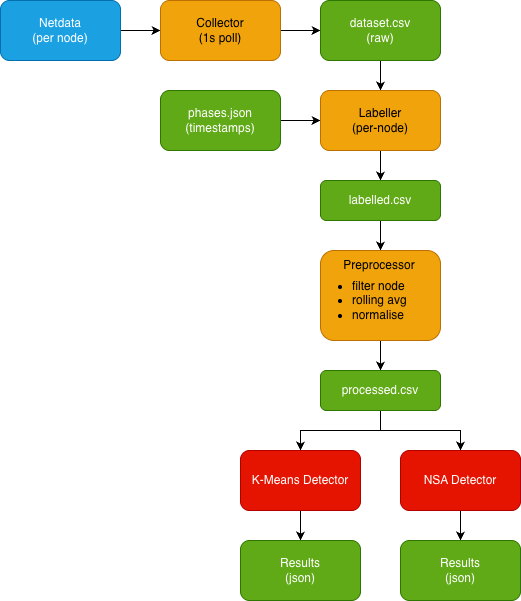
\includegraphics[width=0.92\textwidth]{../docs/data-flow.png}
    \caption{Online telemetry data-flow pipeline used in the replication experiment.}
    \label{fig:online-data-flow}
\end{figure}

\subsection{Detection Results}

The detectors were configured to match the online normalised feature space. NSA used 300 detectors with a radius of 0.15, calibrated for the min-max normalised 0--1 feature range; this differs from the offline configuration (200 detectors, radius 1.5) which operated on raw, unnormalised metric values. K-means used $k = 2$ with an anomaly threshold of mean distance plus two standard deviations, computed on the training (baseline) data.

Tables~\ref{tab:worker-results-2} and~\ref{tab:worker-results-3} present precision, recall, and F1 for each detector and window size on each worker node.

\begin{table}[h]
    \centering
    \begin{tabular}{llllll}
        \hline
        \textbf{Window} & \textbf{Detector} & \textbf{Accuracy} & \textbf{Precision} & \textbf{Recall} & \textbf{F1} \\
        \hline
        3  & K-Means & 0.775 & 0.00  & 0.000 & 0.000 \\
        3  & NSA     & 0.981 & 1.00  & 0.897 & 0.946 \\
        5  & K-Means & 0.780 & 0.00  & 0.000 & 0.000 \\
        5  & NSA     & 0.976 & 1.00  & 0.872 & 0.932 \\
        10 & K-Means & 0.880 & 0.733 & 0.564 & 0.638 \\
        10 & NSA     & 0.986 & 1.00  & 0.923 & 0.960 \\
        \hline
    \end{tabular}
    \caption{Detection results for k3s-worker-2 across window sizes.}
    \label{tab:worker-results-2}
\end{table}

\begin{table}[h]
    \centering
    \begin{tabular}{llllll}
        \hline
        \textbf{Window} & \textbf{Detector} & \textbf{Accuracy} & \textbf{Precision} & \textbf{Recall} & \textbf{F1} \\
        \hline
        3  & K-Means & 0.749 & 0.00 & 0.000 & 0.000 \\
        3  & NSA     & 0.991 & 1.00 & 0.960 & 0.980 \\
        5  & K-Means & 0.739 & 0.00 & 0.000 & 0.000 \\
        5  & NSA     & 0.991 & 1.00 & 0.960 & 0.980 \\
        10 & K-Means & 0.725 & 0.00 & 0.000 & 0.000 \\
        10 & NSA     & 0.981 & 1.00 & 0.920 & 0.958 \\
        \hline
    \end{tabular}
    \caption{Detection results for k3s-worker-3 across window sizes.}
    \label{tab:worker-results-3}
\end{table}

\subsection{Analysis}

The online results confirm and extend the key findings of the offline evaluation. NSA substantially outperforms K-means across all configurations on both worker nodes, consistent with the conclusions of Fritzsche et al.~\cite{fritzsche2024lightweight}.

K-means failed to detect any anomalies at window sizes 3 and 5, achieving precision, recall, and F1 of zero despite correct-majority accuracy (reflecting the class imbalance between normal and anomalous timestamps). At window size 10, K-means recovered to F1 = 0.638 on worker-2 but still produced zero detections on worker-3. This behaviour is consistent with the distance-threshold mechanism: K-means computes an anomaly threshold from baseline distance statistics, and at small window sizes, real telemetry is sufficiently noisy that the variance of baseline distances is large, pushing the threshold above the distances observed during stress phases. The wider smoothing at window size 10 suppresses this variance, allowing the threshold to be crossed, but the improvement is inconsistent across nodes and stress patterns.

NSA achieved near-perfect precision of 1.0 across all configurations, meaning every flagged observation was a genuine anomaly. Recall varied with window size for worker-2 (0.897, 0.872, and 0.923 at windows 3, 5, and 10 respectively) but was stable at 0.960 for worker-3 at windows 3 and 5, dropping only slightly to 0.920 at window 10. The strong and consistent performance of NSA on worker-3 is notable: that node was subjected to a mixed CPU and memory stress, which creates a more pronounced multi-dimensional deviation from the self set, giving NSA a clear non-self region to identify regardless of smoothing level.

Comparing across window sizes, there is no monotonic improvement in NSA recall as the window increases---window 3 and window 10 both achieve high recall on worker-2, while window 5 is marginally weaker. This suggests that for real telemetry, the relationship between window size and anomaly separability is less deterministic than in the synthetic offline case, where the noise-to-signal ratio could be controlled precisely. The offline finding that smaller windows preserve anomaly separability still holds in the sense that NSA at window 3 achieves strong detection (F1 = 0.946 and 0.980) without requiring the heavy smoothing that incapacitates K-means.

Real Netdata telemetry is inherently noisier than synthetic normal-distribution data, introducing greater baseline variance and reducing the geometric distance between normal and stressed operating regions. Despite this, NSA's F1 scores on real cluster data (0.946--0.980) exceeded the offline sustained-anomaly result (0.48 precision) achieved under optimal conditions with a window of 2. This reflects the severity of the stress injected: 120-second, multi-resource stress phases produce deviations that are geometrically unambiguous in the normalised feature space, making the online task considerably more tractable than the offline subtle-anomaly case.

\subsection{Summary}

The online replication demonstrates that the lightweight anomaly detection pipeline of Fritzsche et al.~\cite{fritzsche2024lightweight} performs effectively on real K3s cluster telemetry. NSA achieved near-perfect precision at all window sizes, with the best overall configuration being NSA with a window size of 3, yielding F1 scores of 0.946 and 0.980 on the two worker nodes. K-means proved unreliable on real metrics, successfully detecting anomalies only under heavier smoothing and only on one of the two nodes. Based on these results, NSA with a rolling window of 3 was carried into scheduler-side anomaly-source comparison (NSA, z-score, K-means), where NSA was retained as the selected anomaly source for anomaly-aware policy evaluation in Chapter~\ref{chapter3}.